\chapter{Propuesta} \label{sec:propuesta}

\section{Propuesta Técnica}

\begin{figure}[h]
  \label{propuesta}
  \centering
  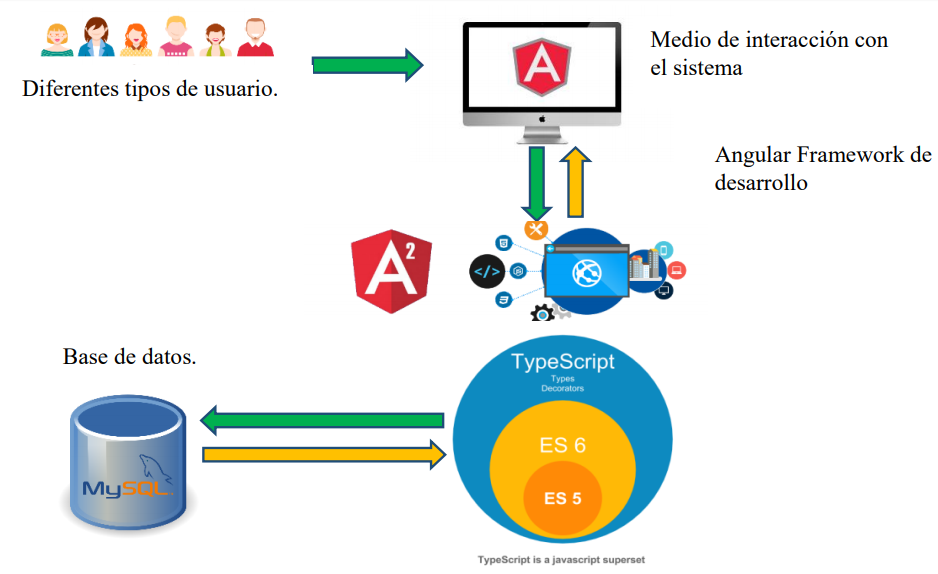
\includegraphics[scale=.5]{lib/assets/propuesta-tecnica}
  \caption{Propuesta Técnica}
\end{figure}

\section{Impácto}
\subsection{Impácto Social}

Según estimaciones oficiales, la aplicación del ECE podría representar el ahorro de 38 mil millones de pesos para el sistema de salud, debido a que se contrarrestarían posibles negligencias médicas, retrasos en la atención, cirugías, robo y desperdicio de medicamento, entre otros. Esto debido a que la falta de información clínica retrasa la atención y puede ser la causa de errores médicos. Esta evolución tecnológica permitirá aumentar la productividad en 20 por ciento; reducir los tiempos y días de espera para consultar en 60 por ciento y ahorros de hasta el 80 por ciento en papelería; reducir los tiempos para cirugía que llegan a ser de hasta 62 días, así como disminuir el desperdicio de medicamento. Además de colocar a México a la altura de otros países que ya implementan este mecanismo. Manual del Expediente Clínico Electrónico. Dirección General de Información en Salud. Secretaría de Salud. México, 2011.
Pacientes con estabilidad respiratoria, hemodinámica y neurológica, el tiempo de espera máximo debe ser de 60 minutos; y verde, pacientes con estabilidad respiratoria, hemodinámica y neurológica, con aspecto saludable y sin riesgo evidente de complicaciones, el tiempo de espera es de hasta cuatro horas. (Chiapas, 2017)
La implementación de un expediente clínico en el estado de Chiapas representaría un gran ahorro económico, tiempo y así como agilizar la atención de cada uno de los pacientes. Actualmente el tiempo de espera para los pacientes en los hospitales llega a ser de cuatro horas, siendo este demasiado tiempo, el cual las personas pudiesen ocupar para realizar sus actividades económicas ya que en el estado un gran porcentaje de la población vive al día con lo poco que gana durante una jornada laborar, siendo esta de una ganancia no estable. Se espera reducir el tiempo de espera en un 80\% con el expediente clínico electrónico.

\subsection{Impácto Tecnológico}
El impácto Tecnológico principal del proyecto será que se desarrolle a las necesidades de la secretaria de salud del estado de Chiapas, siendo una de estas que funcione de manera online y offline, además que pueda contar con una gran escalabilidad ya que es pensado para manejar grandes cantidades de información, datos estadísticos y por supuesto con la mayor seguridad posible.  Con ello se pretende eliminar en su mayoría la duplicidad de los datos o la perdida da de los mismos. Además, se ayudará a aplicar acciones preventivas en la población. Se tendrá un acceso más rápido a la información para la ayuda de investigaciones y desarrollo de la salud en el estado.

\section{Método a desarrollar}
    \subsection{}
      \subsection{}

\section{Angular }
Angular es un Framework desarrollado por los ingenieros de Google, el cual está basado en programación por componentes, los cuales son muy útiles ya que ayudan a reducir grandes cantidades de código reutilizando los componentes en todo el proyecto, pudiendo así tener un mejor control de proyectos de gran escalabilidad. El desarrollo de este sistema tendrá un gran reto que será justamente el control y seguridad de los datos de los pacientes, por ello se decidió utilizar Angular, el cual es un framework muy maduro y con una enorme comunidad que contribuye a su desarrollo. Cuenta con una documentación muy vasta, facilitando así un mejor y óptimo desarrollo, ahorrando tiempo, esfuerzo y además es fácil su despliegue en los servidores. \cite{Angular}

\section{Bulma}
Bulma un framework CSS basado en Flexbox. Una hoja de estilos con diseños predefinidos, basándose en las líneas de diseño propuestas por Google en Material Design.
Ocuparemos de Bulma en el proyecto para el desarrollo de las vistas que interactuaran con el usuario final, teniendo esta una interfaz más agradable y amigable, además como las líneas de diseño están predefinidas, nos ahorraremos mucho tiempo y su interacción con el framework es muy buena. \cite{Bulma}

\section{ Mysql}
Base de datos relacional de código abierto, el cual se trabaja con SQL (Structured Query Language).
El utilizar MySql en el proyecto se debe a que es uno de los mejores gestores con mejor rendimiento, los bajos requisitos para poder ejecutarse, la facilidad de configuración, gran compatibilidad con muchos sistemas operativos, además es uno de los más seguros y la interacción con Angular es fantástica. \cite{mysql}

\section{Typescript}
Es un superset de javascript el cual funciona muy bien con proyectos de gran tamaño, la característica principal del typescript es que reduce significativamente el tamaño del código y lo vuelve a este mucho más comprensible y es el lenguaje que Angular ha adoptado en su esquema de desarrollo.
\subsection{¿Qué es un superset?}

Se trata de un lenguaje escrito sobre otro lenguaje. En este caso Typescript es eso, un lenguaje basado en el original, ofreciéndonos grandes beneficios como el descrito anteriormente, aunque existen otros beneficios. Por ejemplo, mientras otros superset de JavaScript nos alejan del código original, Typescript, por el contrario, es muy similar a Javascript y a C# gracias a que su creador posee conocimientos de ambos lenguajes \cite{typeScript}
